\section{Présentation de l'interface et des outils}
\begin{frame}{L'interface}
	\begin{overprint}
	\begin{enumerate}
		\only<1>{
			\item[]
				\begin{figure}
				    \centering
				    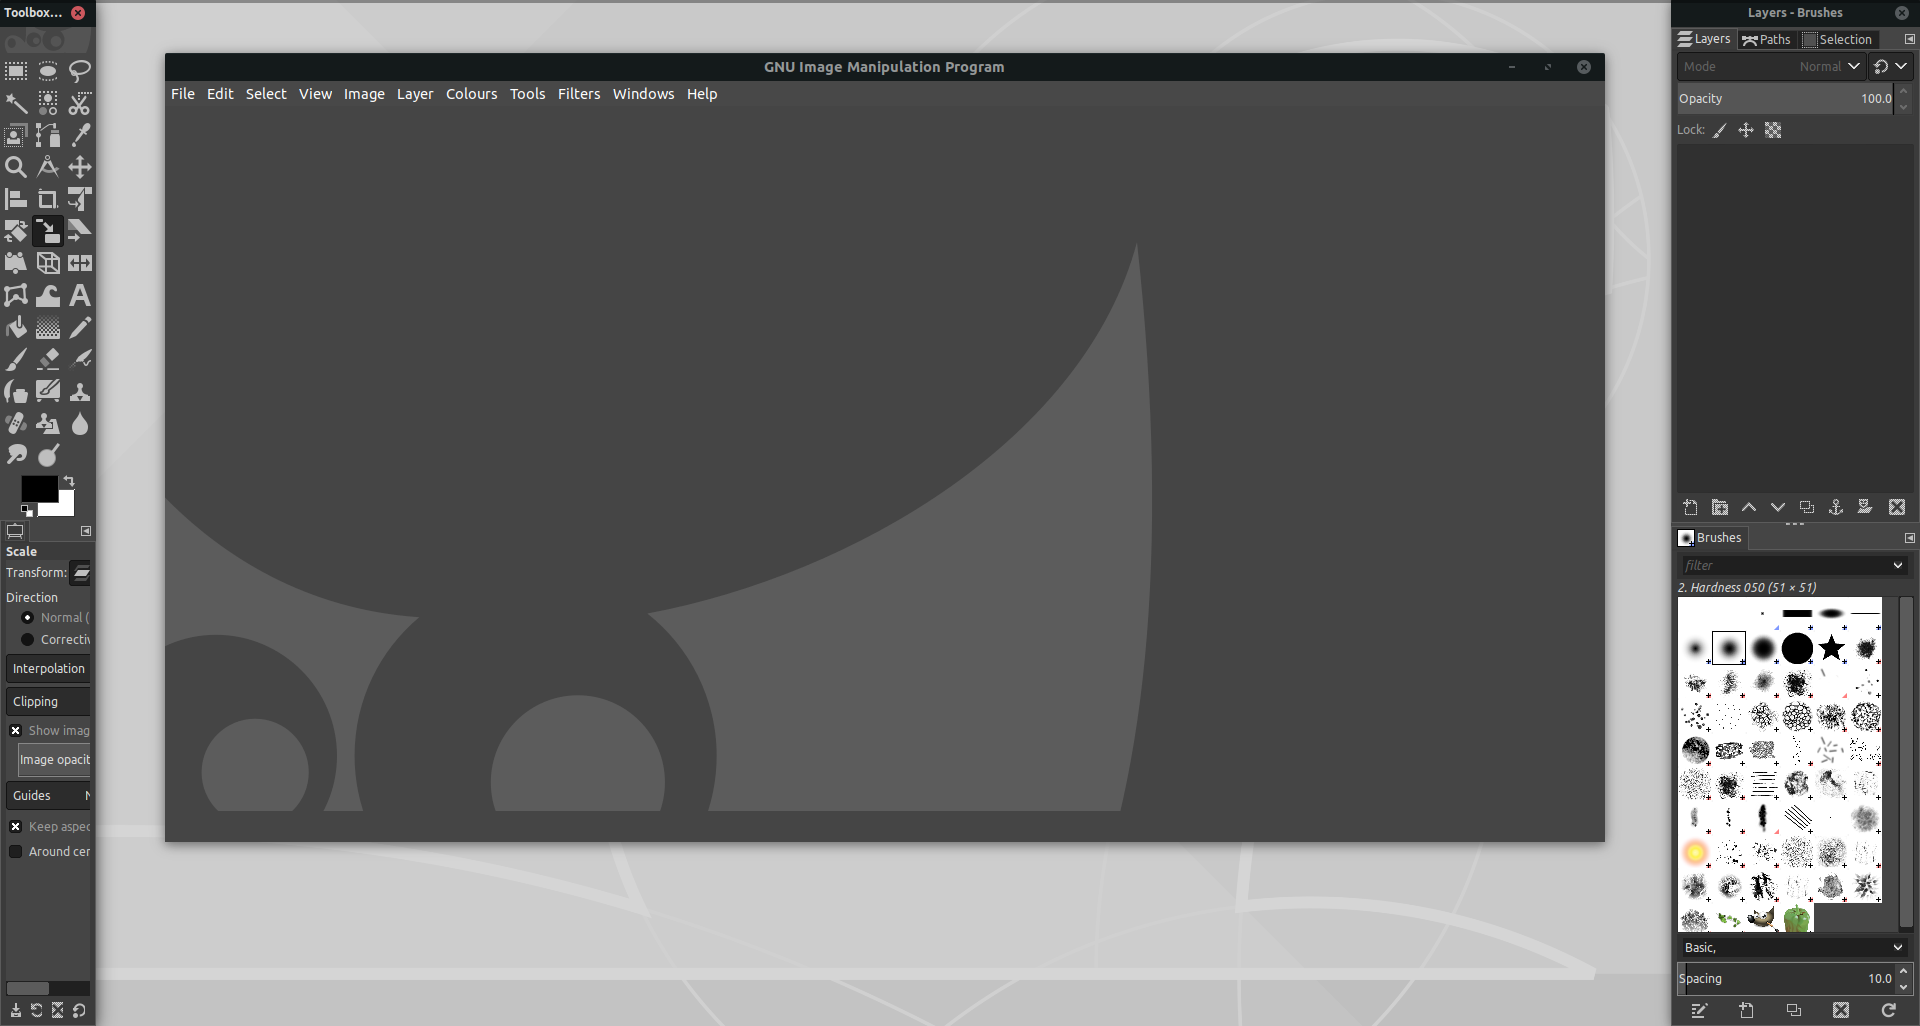
\includegraphics[width=0.9\textwidth]{Images/gimp_multiple_windows}
				    \caption{L'interface multi-fenêtres}
				\end{figure}
		}
		\only<2>{
			\item[]
				\begin{center}
				    Fenêtres > Mode fenêtre unique
				    \begin{figure}
				        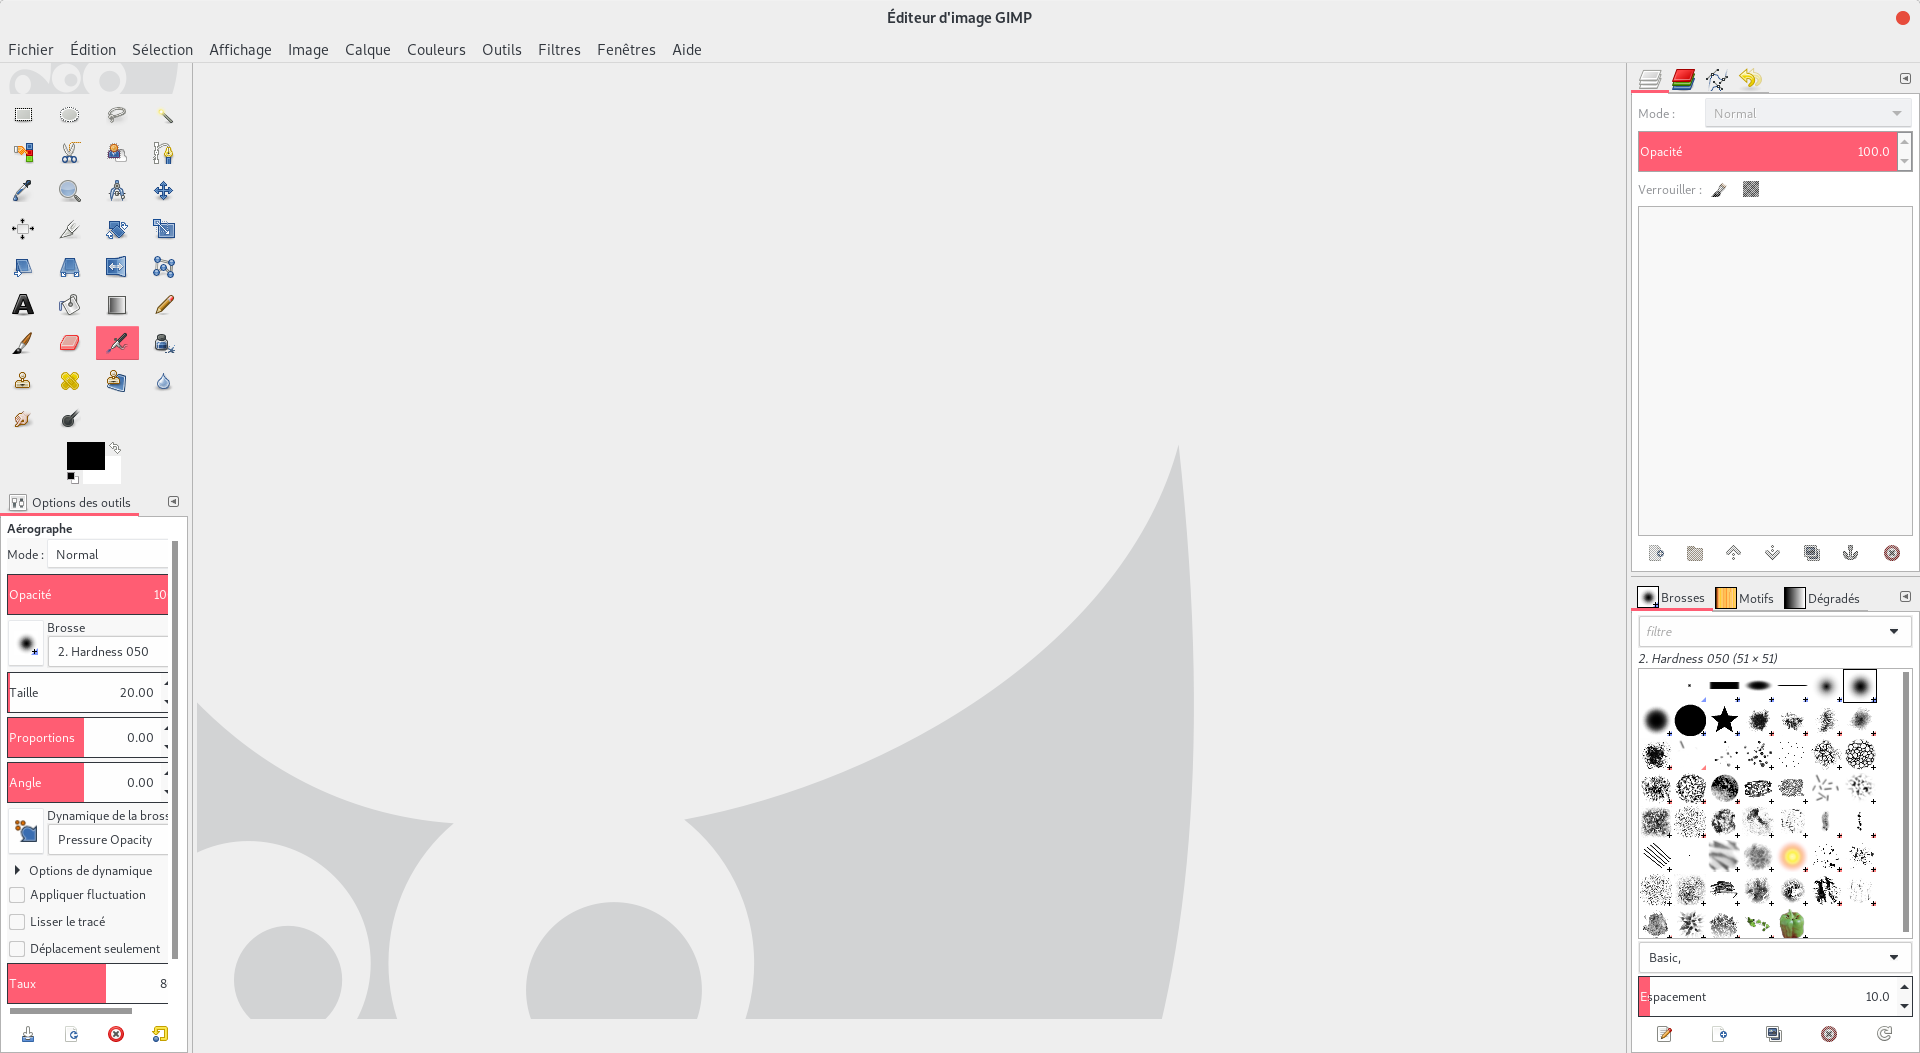
\includegraphics[width=0.9\textwidth]{Images/gimp_single_window}
				        \caption{L'interface fenêtre unique}
				    \end{figure}
				\end{center}
		}
	\end{enumerate}
	\end{overprint}
\end{frame}

\begin{frame}{Créer/importer une image}
	\begin{itemize}
		\item Pour \textbf{créer} une image: Fichier > Nouvelle image ou \keys{\ctrl + N}
			\begin{itemize}
				\item Sélectionnez un modèle (A3, A4, A5...) ou spécifier manuellement les dimensions (en pixels, mm, cm...).
			\end{itemize}
		\item Pour \textbf{importer} une image: Fichier  > Ouvrir ou \keys{\ctrl + O}.
			\begin{itemize}
				\item GIMP supporte de nombreux formats: PNG, JPEG, GIF...
			\end{itemize}
		\item Pour \textbf{créer} depuis le presse-papiers (copier/coller): Créer > Depuis le presse-papiers ou \keys{\shift + \ctrl + V}
	\end{itemize}
	\begin{center}
		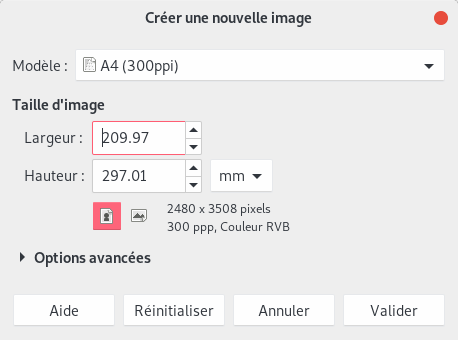
\includegraphics[width=0.5\textwidth]{Images/new_image.png}
	\end{center}
\end{frame}

\begin{frame}{Une image c'est quoi ?}
	\begin{center}
		\textbf{Image matricielle} $\leftrightarrow$ Image vectorielle
		
\includegraphics[width=0.6\textwidth]{Images/mat_vs_vec}
	\end{center}
	Pourquoi n'utilise-t-on pas toujours des images vectorielles ?
	\begin{itemize}
		\item les images vectorielles ne peuvent afficher que des images construites à l'aide de formes. Les images matricielles ont l'avantage d'être définies au pixel près.
	\end{itemize}
\end{frame}

\begin{frame}{Les formats}
	Stocker chaque pixel demande beaucoup de mémoire. Solution ? Compresser les images:
	\begin{itemize}
		\item compression sans pertes (PNG, GIF);
		\item compression avec pertes (JPEG).
	\end{itemize}
	Les trois principaux formats d'images sont
	\begin{itemize}
		\item \textbf{JPEG}: léger (mais avec pertes), idéal pour les photos;
		\item \textbf{PNG}: plus lourd que JPEG (mais sans pertes), très bon support de la transparence;
		\item \textbf{GIF}: support des animations, limité à 256 couleurs.
	\end{itemize}
	Un projet GIMP sera sauvegardé au format \textbf{XCF}, un format d'image libre qui contiendra les différents calques et paramètres de votre création.

	L'équivalent d'Adobe Photoshop est le format \textbf{PSD}.
\end{frame}

\begin{frame}{Enregistrement et exportation}
	\begin{itemize}
		\item Pour \textbf{enregistrer} au format \textbf{XCF}: Fichier > Enregistrer ou \keys{\ctrl + S}.
		\item Pour \textbf{exporter} votre image dans un autre format: Fichier > Exporter ou \keys{\shift + \ctrl + E}.
	\end{itemize}
	\begin{center}
		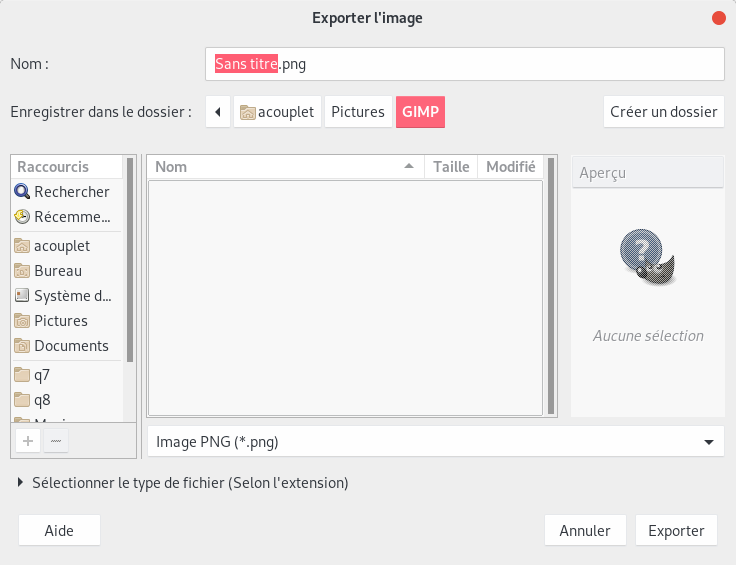
\includegraphics[width=0.5\textwidth]{Images/export}
	\end{center}
\end{frame}

\begin{comment}
\begin{frame}{Les couleurs}
	Il est possible de gérer 2 couleurs: les couleurs de premier et d'arrière-plan:
	\begin{center}
		
\includegraphics[width=0.08\textwidth]{Images/color_primary}
	\end{center}
	Il suffit de cliquer sur une de ces couleurs pour la modifier:
	\begin{center}
		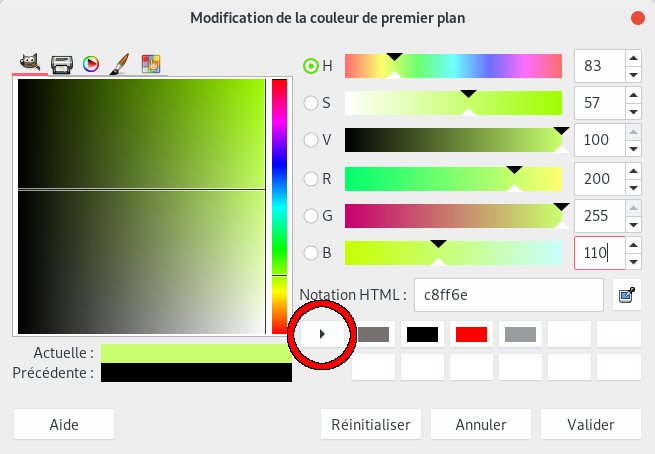
\includegraphics[width=0.5\textwidth]{Images/color_selector}
	\end{center}
	Il est possible de sélectionner une couleur ou de rentrer ses valeurs RGB. Une fois votre couleur choisie, vous pouvez l'ajouter à votre palette.
\end{frame}

\begin{frame}[allowframebreaks]{Les outils de coloration}
	La \textbf{pipette} permet de récupérer la couleur d'un pixel d'une image en cliquant sur le pixel en question.
	\begin{center}
		
\includegraphics[width=0.05\textwidth]{Images/color_tool_0}
		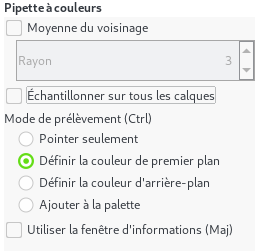
\includegraphics[width=0.3\textwidth]{Images/color_tool_0_settings}
	\end{center}
	L'outil permet de définir la couleur de premier plan, la couleur d'arrière-plan ou simplement d'ajouter la couleur à la palette.

	\framebreak
	Le \textbf{pot de peinture} permet de remplir une zone.
	\begin{center}
		
\includegraphics[width=0.05\textwidth]{Images/color_tool_1}
		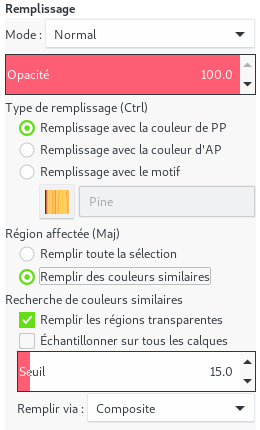
\includegraphics[width=0.25\textwidth]{Images/color_tool_1_settings}
	\end{center}
	Le seuil permet d'ajuster la zone à remplir:
	\begin{center}
		
\includegraphics[width=0.3\textwidth]{Images/color_tool_1_test0}
		
\includegraphics[width=0.3\textwidth]{Images/color_tool_1_test1}
		
\includegraphics[width=0.3\textwidth]{Images/color_tool_1_test2}
	\end{center}
	\begin{scriptsize}
	Exemple: image originale, remplissage noir avec seuil à 30, remplissage noir avec seuil à 60.
	\end{scriptsize}

	\framebreak
	L'outil de gradient permet de créer des dégradés entre la couleur de premier plan et celle d'arrière-plan.
	\begin{center}
		
\includegraphics[width=0.05\textwidth]{Images/color_tool_2}
		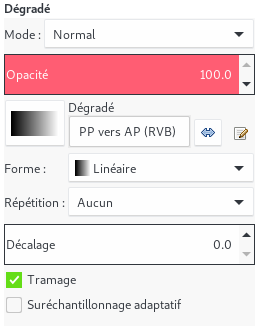
\includegraphics[width=0.3\textwidth]{Images/color_tool_2_settings}
	\end{center}
	Il existe de nombreux modes et de nombreuses formes, n'hésitez pas à les essayer pour les découvrir.

\end{frame}
\end{comment}

\begin{frame}{}
	\begin{overprint}
	\begin{enumerate}

		\only<1>{
			\item[]
				\begin{figure}
				    	\centering
				    	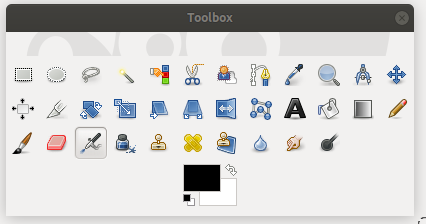
\includegraphics[width=0.4\textwidth]{Images/gimp_toolbox}
				    	\caption{La boîte à outils de GIMP}
					\end{figure}

				\textbf{Accès}

				\begin{itemize}
					\item Fenêtres > Boîte à outils
					\item Outils > Boîte à outils
				\end{itemize}

				\vspace{0.2cm}
				\textbf{Raccourci} \keys{\ctrl + B}
		}

		\only<2>{
			\item[]
				\textbf{Paramètres} \textit{double} cliquer sur l'icône de l'outil concerné
				\begin{figure}
			    	\centering\
			    	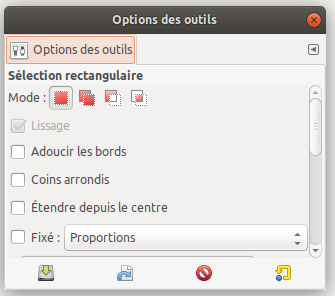
\includegraphics[width=0.4\textwidth]{Images/option_outil}
			    	\caption{Exemple : paramètres de l'outil de sélection}
				\end{figure}
		}

	\end{enumerate}
	\end{overprint}
\end{frame}

\begin{frame}{Les outils de sélection}
\begin{overprint}
\begin{enumerate}

	\only<1>{
		\item[]
			\tool{Rectangulaire}{R}{rectangle.png}
			\vspace{0.5cm}
			\begin{minipage}[t]{0.45\textwidth}
			Options (\textit{fixé}) :

			\begin{itemize}
				\item Position
				\item Proportions fixées
				\item Hauteur fixée
				\item Largeur fixée
			\end{itemize}
			\end{minipage}
			\begin{minipage}[t]{0.45\textwidth}

			\begin{figure}
			    	\centering
			    	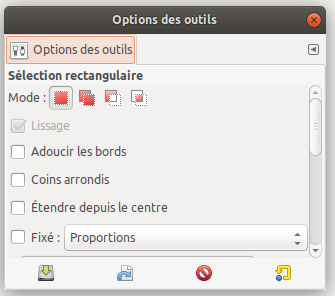
\includegraphics[width=\textwidth]{Images/option_outil}
			\end{figure}
			\end{minipage}

	}

	\only<2>{
		\item[]
			\tool{Elliptique}{E}{ellipse.png}

			\vspace{0.5cm}
			\begin{minipage}[t]{0.45\textwidth}
			Options (\textit{fixé}) :

			\begin{itemize}
				\item Position
				\item Proportions fixées
				\item Hauteur fixée
				\item Largeur fixée
			\end{itemize}
			\end{minipage}
			\begin{minipage}[t]{0.45\textwidth}

			\begin{figure}
			    	\centering
			    	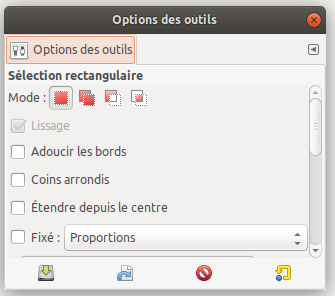
\includegraphics[width=\textwidth]{Images/option_outil}
			\end{figure}
			\end{minipage}
	}
	\only<3>{
		\item[]
			\tool{Ciseaux intelligents}{I}{smart_cut.png}

			\begin{minipage}{0.45\textwidth}
			\begin{figure}
			    	\centering
			    	
\includegraphics[width=\textwidth]{Images/gimp-logo.png}
			\end{figure}
			\end{minipage}\hfill
			\begin{minipage}{0.45\textwidth}
			\begin{figure}
			    	\centering
			    	
\includegraphics[width=\textwidth]{Images/smart_ex.png}
			\end{figure}
			\end{minipage}

			\vspace{0.4cm}
			\textbf{Attention} Une fois le contour terminé, cliquer au \textbf{centre} de celui-ci pour le valider

	}
	\only<4>{
		\item[]
			\tool{À main levée}{F}{freeSelect.png}

			\begin{itemize}
				\item \textbf{Trait continu} Maintenir le clic gauche
			\end{itemize}

			\begin{minipage}{0.45\textwidth}
			\begin{figure}
		    		\centering
		    		
\includegraphics[width=\textwidth]{Images/gimp-logo.png}
			\end{figure}
			\end{minipage}\hfill
			\begin{minipage}{0.45\textwidth}
			\begin{figure}
		    		\centering
		    		
\includegraphics[width=\textwidth]{Images/main_levee.png}
			\end{figure}
			\end{minipage}

	}
	\only<5>{
		\item[]
			\setcounter{enumi}{3}
			\tool{À main levée}{F}{freeSelect.png}

			\begin{itemize}
				\item \textbf{Point par point} Clic pour chaque point successif
			\end{itemize}

			\begin{minipage}{0.45\textwidth}
			\begin{figure}
		    		\centering
		    		
\includegraphics[width=\textwidth]{Images/gimp-logo.png}
			\end{figure}
			\end{minipage}\hfill
			\begin{minipage}{0.45\textwidth}
			\begin{figure}
		    		\centering
		    		
\includegraphics[width=\textwidth]{Images/point_point.png}
			\end{figure}
			\end{minipage}
	}
	\only<6>{
		\item[]
			\tool{Par couleur}{Maj + 0}{colorSelect}

			\vspace{0.3cm}
			\begin{minipage}[t]{0.55\textwidth}
				Options :

				\begin{itemize}
					\item Mode de sélection
					\item Seuil
					\item Echantillonner sur tous les calques
				\end{itemize}
			\end{minipage}
			\begin{minipage}[t]{0.35\textwidth}

				\begin{figure}
			    		\centering
			    		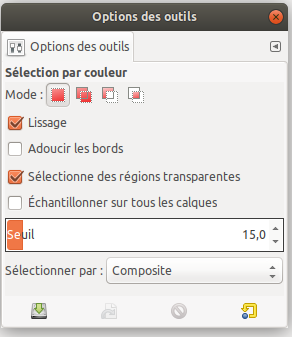
\includegraphics[width=\textwidth]{Images/opt_color_select}
				\end{figure}
			\end{minipage}
	}
	\only<7>{
		\item[]
			\setcounter{enumi}{4}
			\tool{Par couleur}{Maj + 0}{colorSelect}

			\begin{minipage}{0.45\textwidth}

			\begin{figure}
		    		\centering
		    		
\includegraphics[width=\textwidth]{Images/gimp-logo.png}
		    		\caption{Figure originelle}
			\end{figure}
			\end{minipage}\hfill
			\begin{minipage}{0.45\textwidth}
			\begin{figure}
		    		\centering
		    		
\includegraphics[width=\textwidth, trim = 0 0.22cm 0 0, clip]{Images/color_ex.png}
		    		\caption{Zone sélectionnée (en \textbf{rouge})}
			\end{figure}
			\end{minipage}
	}

\end{enumerate}
\end{overprint}
\end{frame}

\begin{frame}{Les outils de sélection}
\textbf{Paramètres de sélection}
\begin{figure}
	    \centering
	    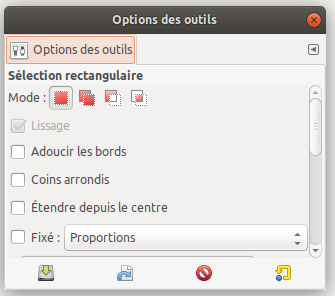
\includegraphics[width=0.4\textwidth]{Images/option_outil}
\end{figure}

\begin{enumerate}
	\item \textbf{Remplacer} la sélection actuelle
	\item \textbf{Ajouter} à la sélection actuelle
	\item \textbf{Soustraire} à la sélection actuelle
	\item \textbf{Intersection} avec la sélection actuelle
\end{enumerate}
\end{frame}

\begin{frame}{Les outils de sélection}
\textbf{Paramètres de sélection}
\begin{overprint}
\begin{figure}
	    \centering
	    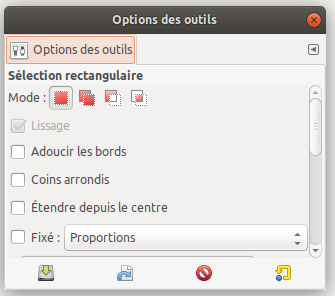
\includegraphics[width=0.4\textwidth, trim = 0 6.3cm 0 0, clip]{Images/option_outil}
\end{figure}

\begin{enumerate}

	\only<1>{
	\item \textbf{Exemple}
	\begin{figure}
	    	\centering
	    	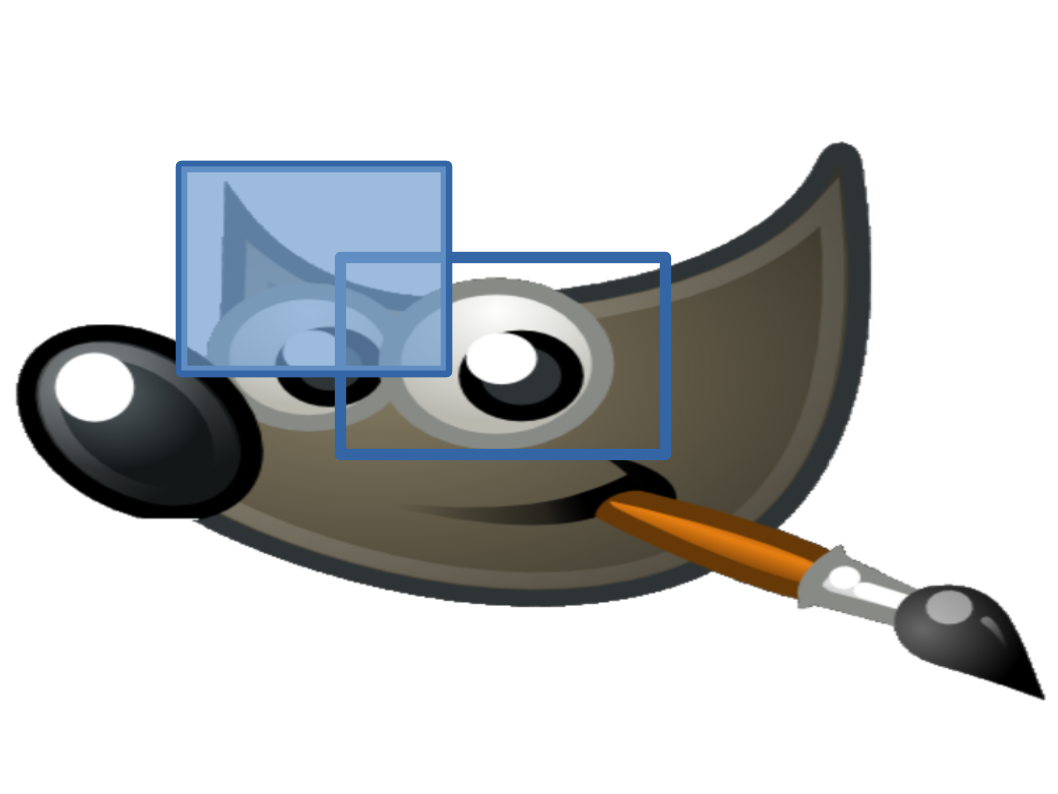
\includegraphics[width=0.4\textwidth]{Images/Selec1.png}
	\end{figure}}

	\only<2>{
	\item[1] \textbf{Remplacer} la sélection actuelle
	\begin{figure}
	    	\centering
	    	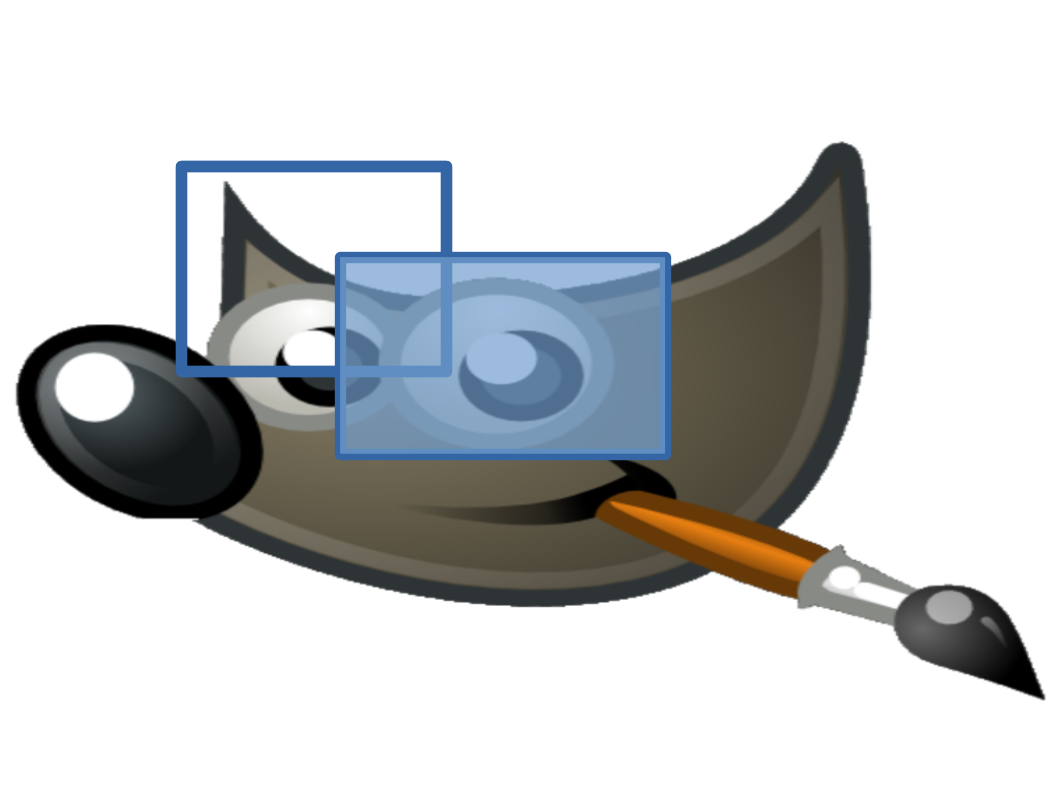
\includegraphics[width=0.4\textwidth]{Images/Selec5.png}
	\end{figure}}

	\only<3>{
	\item[2] \textbf{Ajouter} à la sélection actuelle
	\begin{figure}
	    	\centering
	    	
\includegraphics[width=0.4\textwidth]{Images/Selec2.png}
	\end{figure}}

	\only<4>{
	\item[3] \textbf{Soustraire} à la sélection actuelle
	\begin{figure}
	    	\centering
	    	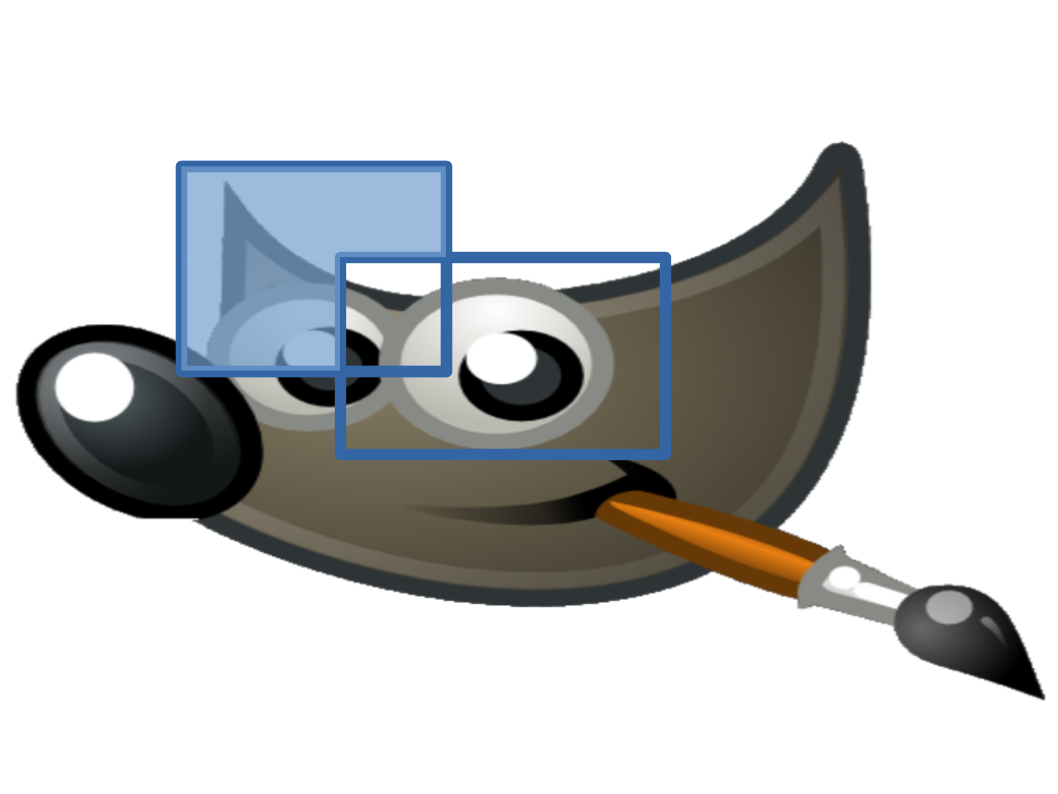
\includegraphics[width=0.4\textwidth]{Images/Selec3.png}
	\end{figure}}

	\only<5>{
	\item[4] \textbf{Intersection} avec la sélection actuelle
	\begin{figure}
	    	\centering
	    	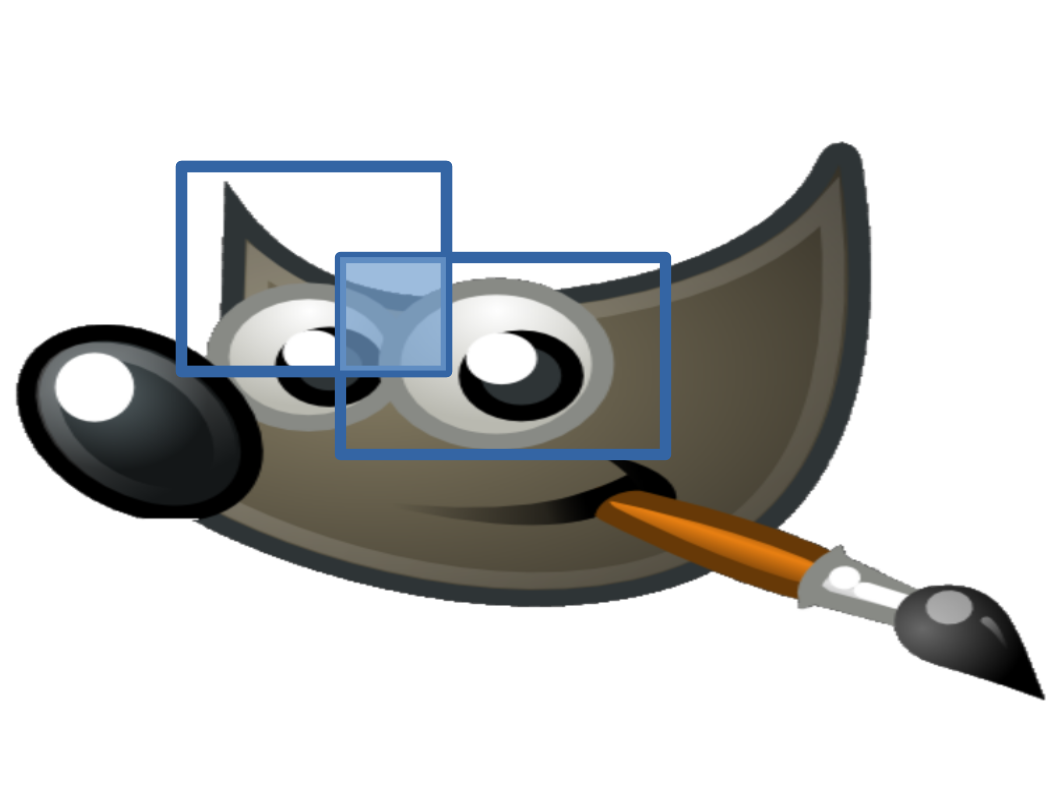
\includegraphics[width=0.4\textwidth]{Images/Selec4.png}
	\end{figure}}

\end{enumerate}
\end{overprint}
\end{frame}

\begin{frame}{Les outils de transformation}

	\begin{overprint}
	\begin{enumerate}

		\only<1>{
			\item[]
				\tool{Rotation}{Maj+R}{rotate.png}
				\vspace{0.5cm}

				\begin{minipage}{0.45\textwidth}
				\begin{figure}
				    	\centering
				    	
\includegraphics[width=\textwidth]{Images/gimp-logo.png}
				\end{figure}
				\end{minipage}\hfill
				\begin{minipage}{0.45\textwidth}
				\begin{figure}
				    	\centering
				    	
\includegraphics[width=0.8\textwidth]{Images/Rotate.png}
				\end{figure}
				\end{minipage}
		}

		\only<2>{
			\item[]
				\tool{Agrandissement/Réduction}{Maj+T}{rescale.png}

				\begin{minipage}{0.45\textwidth}
				\begin{figure}
				    	\centering
				    	
\includegraphics[width=\textwidth]{Images/gimp-logo.png}
				\end{figure}
				\end{minipage}\hfill
				\begin{minipage}{0.45\textwidth}
				\begin{figure}
				    	\centering
				    	
\includegraphics[width=\textwidth]{Images/redimension.png}
				\end{figure}
				\end{minipage}
		}

		\only<3>{
			\item[]
				\tool{Inversion}{Maj+F}{flip.png}

				\begin{minipage}{0.45\textwidth}
				\begin{figure}
				    	\centering
				    	
\includegraphics[width=\textwidth]{Images/gimp-logo.png}
				\end{figure}
				\end{minipage}\hfill
				\begin{minipage}{0.45\textwidth}
				\begin{figure}
				    	\centering
				    	
\includegraphics[width=\textwidth]{Images/Flip.png}
				\end{figure}
				\end{minipage}
		}

		\only<4>{
			\item[]
				\setcounter{enumi}{2}
				\tool{Inversion}{Maj+F}{flip.png}

				\begin{minipage}{0.45\textwidth}
				\begin{figure}
				    	\centering
				    	
\includegraphics[width=\textwidth]{Images/gimp-logo.png}
				\end{figure}
				\end{minipage}\hfill
				\begin{minipage}{0.45\textwidth}
				\begin{figure}
				    	\centering
				    	
\includegraphics[width=\textwidth]{Images/Flip2.png}
				\end{figure}
				\end{minipage}
		}
		\only<5>{
			\item[]
				\tool{Cisaillement}{Maj+S}{shear.png}
				\vspace{0.5cm}

				\begin{minipage}{0.45\textwidth}
				\begin{figure}
				    	\centering
				    	
\includegraphics[width=0.8\textwidth]{Images/NoShear.png}
				\end{figure}
				\end{minipage}\hfill
				\begin{minipage}{0.45\textwidth}
				\begin{figure}
				    	\centering
				    	
\includegraphics[width=0.8\textwidth]{Images/Shear.png}
				\end{figure}
				\end{minipage}
		}

		\only<6>{
			\item[]
				\tool{Mise en perspective}{Maj+R}{perspective.png}
				\vspace{0.3cm}

				\begin{minipage}{0.45\textwidth}
				\begin{figure}
				    	\centering
				    	
\includegraphics[width=0.5\textwidth]{Images/FullTex.png}
				\end{figure}
				\end{minipage}\hfill
				\begin{minipage}{0.45\textwidth}
				\begin{figure}
				    	\centering
				    	
\includegraphics[width=0.5\textwidth]{Images/Perspective.png}
				\end{figure}
				\end{minipage}
		}

		\only<7>{
			\item[]
				\tool{Découpe}{Maj+C}{cutTool.png}

				\begin{minipage}{0.45\textwidth}
				\begin{figure}
				    	\centering
				    	
\includegraphics[width=\textwidth]{Images/gimp-logo.png}
				\end{figure}
				\end{minipage}\hfill
				\begin{minipage}{0.45\textwidth}
				\begin{figure}
				    	\centering
				    	
\includegraphics[width=0.6\textwidth]{Images/cut.png}
				\end{figure}
				\end{minipage}
		}
	\end{enumerate}
	\end{overprint}
\end{frame}


\begin{frame}{Les outils de coloration}
	\textbf{Couleurs actives}

	\begin{figure}
		\centering
		\begin{tikzpicture}[scale=0.7, transform shape]
		    \node[anchor=south west,inner sep=0] at (0.4,0) {\includegraphics[width=0.1\textwidth]{Images/gimp_couleurs_actives}};
		    \onslide<2>{\draw[teal,ultra thick,rounded corners] (0.25,0.3) rectangle (1.5,1);
		    \node [anchor=center, teal] (note) at (0.7,1.4) {\Large Avant-plan \textcolor{black}{{\small (Clic \textbf{gauche})}}};}
		\onslide<3>{\draw[red,ultra thick,rounded corners] (0.6,0) rectangle (1.55,0.7);
		    \node [anchor=center, red] (Inner) at (0.7,-0.3) {\Large Arrière-plan \textcolor{black}{{\small (Clic \textbf{droit})}}};}
			\end{tikzpicture}
	\end{figure}

	\vspace{-0.2cm}
	\textbf{Palette des couleurs} Double clique sur l'une des couleurs actives


	\begin{figure}
		\centering
		\begin{tikzpicture}[scale=1, transform shape]
		    \node[anchor=south west,inner sep=0] at (0.4,0) {\includegraphics[width=0.4\textwidth]{Images/gimp_color_box}};

		    \onslide<4>{\draw[red,ultra thick,rounded corners] (4.2,1.2) rectangle (4.6,1.6);
		    \node [anchor=center, red] (note) at (3.7,-0.4) {\Large Sélection de couleur};}
			\end{tikzpicture}
	\end{figure}
\end{frame}


\begin{frame}{Les outils de coloration}
	\begin{minipage}[t]{0.49\textwidth}
		\textbf{Code HTML}

		\vspace{0.2cm}
		Couleurs pré-définies

		\vspace{0.2cm}

		\begin{center}
		\fbox{\parbox{0.7\linewidth}{%
		\url{https://www.toutes-les-couleurs.com/code-couleur-html.php}
		}}
		\end{center}

	\end{minipage}\hfill
	\begin{minipage}[t]{0.49\textwidth}
		\textbf{Code RGB}

		\begin{itemize}
			\item[H] Teinte
			\item[S] Valeur
			\item[V] Saturation
			\item[R] Rouge
			\item[G] Vert
			\item[B] Bleu
		\end{itemize}

	\end{minipage}
\end{frame}


\begin{frame}{Les outils de coloration}
	\begin{overprint}
	\begin{enumerate}
		\only<1>{
			\item[]
				\tool{Sélection de couleur}{O}{colorProbe.png}

				\vspace{0.5cm}
				\tool{Outil de remplissage}{Maj + B}{bucketFill.png}

				\tool{Crayon}{N}{pen.png}

				\tool{Pinceau}{P}{paintbrush.png}

				\tool{Aérograhe}{A}{aero.png}

		}

		\only<2>{
			\item[]
				\tool{Dégradé}{L}{colorTool2.png}

				\begin{minipage}{0.45\textwidth}
				\begin{figure}
				    	\centering
				    	\includegraphics[width=\textwidth]{Images/degrade_ex.png}
				\end{figure}
				\end{minipage}\hfill
				\begin{minipage}{0.45\textwidth}
				\begin{figure}
				    	\centering
				    	\includegraphics[width=\textwidth]{Images/degrade_ex2.png}
				\end{figure}
				\end{minipage}


				Tracer des \textbf{lignes droites} : \textbf{majuscule enfoncée} entre deux points sélectionnés
		}
	\end{enumerate}
	\end{overprint}
\end{frame}

\begin{frame}{Autres outils}
	\begin{overprint}
	\begin{enumerate}
		\only<1>{
			\item[]
				\tool{Zoom}{Z}{zoom.png}

				\textbf{Raccourci} \keys{{+}}, \keys{-}, \keys{1}, \keys{2}, \keys{3}, \keys{4} et \keys{5}
				\vspace{0.6cm}

				\tool{Déplacement}{M}{moove.png}
		}

		\only<2>{
			\item[]
				\tool{Alignement}{Q}{autopose.png}

				\begin{figure}
				    	\centering
				    	\includegraphics[width=0.3\textwidth]{Images/automoove_opt.png}
				\end{figure}
		}
	\end{enumerate}
	\end{overprint}
\end{frame}

\begin{frame}{Les mesures}
	\begin{overprint}
	\begin{enumerate}
		\only<1>{
			\item[]
				\textbf{Echelle graduée} aux \textit{extrémités} de l'image

				\begin{figure}
				    	\centering
				    	\includegraphics[width=0.3\textwidth]{Images/Scale.png}
				    \end{figure}

				\vspace{0.3cm}

				\item Zone de \textbf{"Communication"} dans le \textit{coin inférieur droit}

				\begin{figure}
				    	\centering
				    	\includegraphics[width=0.3\textwidth]{Images/commu.png}
				\end{figure}
		}

		\only<2>{
			\item[]
				\tool{Outil de mesure}{Maj + M}{measure.png}
				\begin{minipage}{0.45\textwidth}
				\begin{figure}
				    	\centering
				    	\includegraphics[width=\textwidth]{Images/gimp-logo.png}
				\end{figure}
				\end{minipage}\hfill
				\begin{minipage}{0.45\textwidth}
				\begin{figure}
				    	\centering
				    	\includegraphics[width=\textwidth]{Images/measure_gimp.png}
				\end{figure}
				\end{minipage}

				\begin{itemize}
					\item \textbf{Maintenir} le clic gauche entre les deux zones de mesure
					\item \textbf{Résultats} dans la zone \textit{inférieure droite} de l'écran
				\end{itemize}
		}
	\end{enumerate}
	\end{overprint}
\end{frame}

\begin{frame}{Les calques}
	\begin{overprint}
	\begin{enumerate}
		\only<1>{
			\item[]
				\begin{figure}
				    	\centering
				    	\includegraphics[width=0.3\textwidth]{Images/gimp_calques}
				\end{figure}

				\textbf{Accès} Fenêtres > Calques

				\vspace{0.2cm}
				\textbf{Raccourci} \keys{\ctrl + L}
		}

		\only<2>{
			\item[]
				\begin{figure}
				    	\centering
				    	\includegraphics[width=0.5\textwidth]{Images/Calque.jpg}
					\end{figure}

				\begin{itemize}
					\item \textbf{Superposition} d'images
					\begin{itemize}
						\item \textit{Avant-plan} : le plus haut
						\item \textit{Arrière-plan} : le plus bas
					\end{itemize}
					\item Visible ou non
					\item Ancrable
					\item Indépendant
				\end{itemize}
		}
	\end{enumerate}
	\end{overprint}
\end{frame}


\begin{frame}{Exercice I}
	\begin{overprint}
	\begin{enumerate}
		\only<1>{
			\item[]
				Image de départ: \href{http://louvainlinux.github.io/atelier-gimp/src/Images/ex1/original.jpg}{Lien de l'image}
				\begin{center}
				\includegraphics[width=0.45\textwidth]{Images/ex1/Ex1_step0.jpg}
				\includegraphics[width=0.45\textwidth]{Images/ex1/Ex1_step5.jpg}
				\end{center}
		}

		\only<2>{
			\item[]
				Découpe de l'image
				\begin{center}
					\includegraphics[width=0.4\textwidth]{Images/ex1/Ex1_step1.jpg}
				\end{center}
		}

		\only<3>{
			\item[]
				Inversion de l'image
				\begin{center}
					\includegraphics[width=0.4\textwidth]{Images/ex1/Ex1_step2.jpg}
				\end{center}
		}

		\only<4>{
			\item[]
				Coloration de zones du ballon en R=237, G=178 et B=35.
				\begin{center}
					\includegraphics[width=0.4\textwidth]{Images/ex1/Ex1_step3.jpg}
				\end{center}

		}

		\only<5>{
			\item[]
				Mise en place d'un cadre
				\begin{center}
					\includegraphics[width=0.4\textwidth]{Images/ex1/Ex1_step4.jpg}
				\end{center}
		}

		\only<6>{
			\item[]
				Texte en rouge
				\begin{center}
					\includegraphics[width=0.4\textwidth]{Images/ex1/Ex1_step5.jpg}
				\end{center}
		}
	\end{enumerate}
	\end{overprint}
\end{frame}
